\documentclass[12pt,a4paper]{article}

% ─── Page Layout ───────────────────────────────────────────────────────────────
\usepackage[a4paper, margin=0.8in, headheight=14pt]{geometry}

% ─── Fonts (XeLaTeX) ───────────────────────────────────────────────────────────
\usepackage{fontspec}
\usepackage{unicode-math}
\setmainfont{TeX Gyre Pagella}
\setmonofont[Scale=0.88]{TeX Gyre Cursor}
\setmathfont{Latin Modern Math}

% ─── Packages ──────────────────────────────────────────────────────────────────
\usepackage{xcolor}
\usepackage{colortbl}
\usepackage{titlesec}
\usepackage{enumitem}
\usepackage{tabularx}
\usepackage{booktabs}
\usepackage{array}
\usepackage{amsmath}
\usepackage{tikz}
\usetikzlibrary{shapes.geometric, arrows.meta, positioning, calc, fit, decorations.pathreplacing}
\usepackage{tcolorbox}
\tcbuselibrary{skins, breakable}
\usepackage{hyperref}
\usepackage{fancyhdr}
\usepackage{graphicx}
\usepackage{microtype}
\hyphenpenalty=10000
\exhyphenpenalty=10000
\sloppy
\usepackage{caption}
\usepackage{setspace}
\usepackage{multirow}
\usepackage{tocloft}

% ─── Q&A helper ────────────────────────────────────────────────────────────────
\newcommand{\Q}[1]{\textbf{#1}\par\noindent\ignorespaces}

% ─── Colour Palette ────────────────────────────────────────────────────────────
\definecolor{myred}{RGB}{196,30,58}
\definecolor{mydark}{RGB}{30,30,50}
\definecolor{mygreen}{RGB}{14,120,80}
\definecolor{myteal}{RGB}{0,130,140}
\definecolor{myamber}{RGB}{180,100,0}
\definecolor{mypurple}{RGB}{100,30,160}
\definecolor{mygray}{RGB}{246,247,249}
\definecolor{mgframe}{RGB}{180,185,200}
\definecolor{watermark}{RGB}{145,150,170}
\definecolor{hdrred}{RGB}{250,232,235}
\definecolor{hdrgreen}{RGB}{220,244,233}
\definecolor{hdrteal}{RGB}{220,242,244}
\definecolor{hdramber}{RGB}{253,242,215}
\definecolor{hdrpurple}{RGB}{238,228,255}
\definecolor{hdrgray}{RGB}{238,240,245}
\definecolor{rowalt}{RGB}{250,251,253}

% ─── Section Formatting ────────────────────────────────────────────────────────
\titleformat{\section}
  {\large\bfseries\color{myred}}{\thesection.}{0.5em}{}
  [\vspace{1pt}{\color{myred}\rule{\linewidth}{0.8pt}}]
\titleformat{\subsection}
  {\normalsize\bfseries\color{myteal}}{\thesubsection}{0.5em}{}
\titlespacing*{\section}{0pt}{18pt}{7pt}
\titlespacing*{\subsection}{0pt}{11pt}{4pt}

% ─── Paragraph ─────────────────────────────────────────────────────────────────
\setlength{\parindent}{0pt}
\setlength{\parskip}{4pt}

% ─── TOC Styling ───────────────────────────────────────────────────────────────
\renewcommand{\cfttoctitlefont}{\large\bfseries\color{myred}}
\renewcommand{\cftaftertoctitle}{\par\noindent{\color{myred}\rule{\linewidth}{0.8pt}}}
\setlength{\cftbeforetoctitleskip}{0pt}
\setlength{\cftaftertoctitleskip}{6pt}
\renewcommand{\cftsecfont}{\normalsize\bfseries\color{mydark}}
\renewcommand{\cftsecpagefont}{\normalsize\bfseries\color{mydark}}
\renewcommand{\cftsecleader}{\cftdotfill{\cftdotsep}}
\setlength{\cftbeforesecskip}{7pt}
\renewcommand{\cftsubsecfont}{\small\color{mydark}}
\renewcommand{\cftsubsecpagefont}{\small\color{mydark}}
\setlength{\cftbeforesubsecskip}{3pt}
\setlength{\cftsubsecindent}{1.4em}

% ─── Table helpers ─────────────────────────────────────────────────────────────
\renewcommand{\arraystretch}{1.45}
\setlength{\tabcolsep}{6pt}
\arrayrulecolor{mydark}
\newcolumntype{B}[1]{>{\small\bfseries\raggedright\arraybackslash}m{#1}}
\newcolumntype{Y}{>{\small\raggedright\arraybackslash}X}
\renewcommand{\tabularxcolumn}[1]{m{#1}}

% ─── Header / Footer ───────────────────────────────────────────────────────────
\pagestyle{fancy}
\fancyhf{}
\fancyhead[L]{\small\color{myred}\textbf{PE-EC701C}\;\color{mydark}--- Mobile Communication and Networks}
\fancyhead[R]{\small\color{myteal}\textbf{Module 1 Notes}}
\fancyfoot[C]{\small\color{mydark}\thepage}
\fancyfoot[R]{\small\color{watermark}\textit{\copyright\ Biraj}}
\renewcommand{\headrulewidth}{0.5pt}
\renewcommand{\footrulewidth}{0.3pt}

% ─── Hyperref ──────────────────────────────────────────────────────────────────
\hypersetup{
  colorlinks=true, linkcolor=myteal, urlcolor=myteal,
  pdfauthor={Biraj Sarkar},
  pdftitle={PE-EC701C --- Module 1 Notes}
}

% ─── tcolorbox styles ──────────────────────────────────────────────────────────
\tcbset{
  tikzbox/.style={
    colback=mygray, colframe=mgframe, boxrule=0.6pt, arc=4pt,
    left=8pt, right=8pt, top=6pt, bottom=6pt,
    colbacktitle=mgframe, coltitle=mydark,
    fonttitle=\small\bfseries
  },
  defbox/.style={
    colback=hdrgreen, colframe=mygreen, boxrule=0.8pt, arc=4pt,
    left=9pt, right=9pt, top=6pt, bottom=6pt,
    colbacktitle=mygreen, coltitle=white,
    fonttitle=\small\bfseries
  },
  formulabox/.style={
    colback=hdrteal, colframe=myteal, boxrule=0.8pt, arc=4pt,
    left=9pt, right=9pt, top=7pt, bottom=7pt,
    colbacktitle=myteal, coltitle=white,
    fonttitle=\small\bfseries
  },
  examplebox/.style={
    colback=hdramber, colframe=myamber, boxrule=0.8pt, arc=4pt,
    left=9pt, right=9pt, top=6pt, bottom=6pt,
    colbacktitle=myamber, coltitle=white,
    fonttitle=\small\bfseries
  },
  masonbox/.style={
    colback=hdrpurple, colframe=mypurple, boxrule=0.8pt, arc=4pt,
    left=9pt, right=9pt, top=6pt, bottom=6pt,
    colbacktitle=mypurple, coltitle=white,
    fonttitle=\small\bfseries
  },
  exambox/.style={
    colback=hdrpurple, colframe=mypurple, boxrule=1pt, arc=5pt,
    left=10pt, right=10pt, top=8pt, bottom=8pt,
    colbacktitle=mypurple, coltitle=white,
    fonttitle=\bfseries,
    breakable, title after break={\textbf{Frequently Asked / Viva Questions (contd.)}}}
}
\tcbset{breakable}

% ─── TikZ styles ───────────────────────────────────────────────────────────────
\tikzset{
  block/.style={rectangle, draw=myteal, fill=hdrteal,
    text width=2.4cm, align=center, minimum height=0.95cm,
    font=\small, rounded corners=3pt, line width=0.7pt},
  redblock/.style={rectangle, draw=myred, fill=hdrred,
    text width=2.4cm, align=center, minimum height=0.95cm,
    font=\small, rounded corners=3pt, line width=0.7pt},
  netnode/.style={rectangle, draw=myteal, fill=hdrteal,
    text width=1.5cm, align=center, minimum height=0.8cm,
    font=\small, rounded corners=3pt, line width=0.7pt},
  sumjunc/.style={circle, draw=myamber, fill=hdramber,
    minimum size=0.62cm, font=\small, line width=0.8pt},
  snode/.style={circle, draw=mypurple, fill=hdrpurple,
    minimum size=0.55cm, font=\footnotesize, line width=0.7pt},
  arrow/.style={-Stealth, thick, color=mydark},
  redarrow/.style={-Stealth, thick, color=myred},
  line/.style={thick, color=mydark},
  hexagon/.style={
    regular polygon, regular polygon sides=6,
    draw=myteal, fill=hdrteal, minimum size=1.8cm, inner sep=0pt,
    line width=0.8pt, rotate=30
  }
}

% ═══════════════════════════════════════════════════════════════════════════════
\begin{document}
% ═══════════════════════════════════════════════════════════════════════════════

\begin{center}
  {\LARGE\bfseries\color{myred} PE-EC701C --- Mobile Communication and Networks}\\[5pt]
  {\normalsize\color{mydark} Semester VII \quad$\bullet$\quad 3L:0T:0P \quad$\bullet$\quad 3 Credits}\\[3pt]
  {\normalsize\color{myteal}\textbf{Module 1 Exam Notes: Cellular Concepts and Wireless Standards}}\\[3pt]
  {\small\color{mydark} CGEC \;$|$\; B.Tech ECE (2023--27) \;$|$\; \textit{Biraj Sarkar}}
\end{center}
\vspace{2pt}
\noindent{\color{myred}\rule{\linewidth}{1.5pt}}
\vspace{2pt}

\hypersetup{linkcolor=mydark}
\tableofcontents
\hypersetup{linkcolor=myteal}
\newpage

% ===============================================================================
\section{Cellular Concepts and Cell Structure}
% ===============================================================================

Early mobile radio systems utilized high-power transmitters on tall towers to achieve maximum coverage. This centralized approach suffered from severe spectral congestion and could support only a handful of simultaneous users. The cellular concept solved this by replacing a single large transmitter with many low-power transmitters distributed across the service area.

\begin{tcolorbox}[defbox]
\textbf{Cellular System:} A system in which a geographical area is partitioned into smaller, adjacent subdivisions called \textbf{cells}, each served by its own low-power base station (BS). By limiting transmitter range, the same frequency channels can be reused by different cells at a safe distance, dramatically increasing network capacity.
\end{tcolorbox}

\subsection{Hexagonal Cell Geometry}
Although real-world cell coverage areas are irregular (due to terrain, buildings, and signal propagation), simplified geometric models are used for system design:
\begin{itemize}[leftmargin=*, itemsep=3pt]
  \item \textbf{Circle:} Represents ideal radiation patterns but cannot be tiled. In overlapping circular configurations, gaps or double-coverage zones occur.
  \item \textbf{Square / Triangle:} Can tile an area without gaps, but the distance from the cell center to its boundary varies heavily, leading to poor cell-edge performance.
  \item \textbf{Hexagon:} The ideal choice. It tiles the plane without gaps or overlaps, closely approximates a circle (ideal omnidirectional radiation), and has the largest area for a given distance to its corners, minimizing the number of cells required to cover a region.
\end{itemize}

% ===============================================================================
\section{Frequency Reuse and Capacity}
% ===============================================================================

Frequency reuse is the core mechanism of cellular systems. It allows a fixed allocation of RF spectrum to support an arbitrary number of users.

\begin{tcolorbox}[defbox]
\textbf{Frequency Reuse:} The design technique of dividing the total available channels into smaller, distinct groups and assigning these groups to different cells, such that cells operating on the same frequency group are physically separated by a distance large enough to keep interference below a tolerable limit.
\end{tcolorbox}

\subsection{Cluster and Geometry Formulation}
Let the total number of duplex channels allocated to the system be $S$. These channels are divided into $N$ orthogonal channel groups, each group containing $k$ channels ($S = k N$).
\begin{itemize}[leftmargin=*, itemsep=2.5pt]
  \item \textbf{Cluster Size ($N$):} The group of $N$ cells that collectively use the entire set of available frequencies. No two cells in a single cluster can share frequencies.
  \item Because of hexagonal geometry constraints, $N$ can only take values that satisfy:
    \begin{equation}
      N = i^2 + ij + j^2 \quad \text{where } i, j \in \{0, 1, 2, \dots\}
    \end{equation}
    Typical values are $N = 1, 3, 4, 7, 9, 12, 19, 21, \dots$
  \item \textbf{System Capacity ($C$):} If a cluster of size $N$ is replicated $M$ times across the system:
    \begin{equation}
      C = M \cdot S = M \cdot k \cdot N
    \end{equation}
\end{itemize}

\subsection{Co-channel Reuse Ratio}
Cells that use the same channel group are called \textbf{co-channel cells}. Let $R$ be the cell radius (distance from center to vertex) and $D$ be the minimum distance between co-channel cell centers.
\begin{tcolorbox}[formulabox, title={\textbf{Co-channel Reuse Distance and Ratio}}]
For a hexagonal grid, the co-channel reuse distance $D$ is given by:
\begin{equation}
  D = R \sqrt{3N}
\end{equation}
The co-channel reuse ratio $Q$ represents the spatial separation normalized by the cell radius:
\begin{equation}
  Q = \frac{D}{R} = \sqrt{3N}
\end{equation}
\textbf{Significance:} A small value of $Q$ implies small cluster size $N$, allowing high frequency reuse and high capacity, but results in higher co-channel interference. A large value of $Q$ reduces interference but lowers capacity.
\end{tcolorbox}

\begin{tcolorbox}[tikzbox, title={7-Cell Frequency Reuse Cluster Pattern (N = 7)}]
\centering
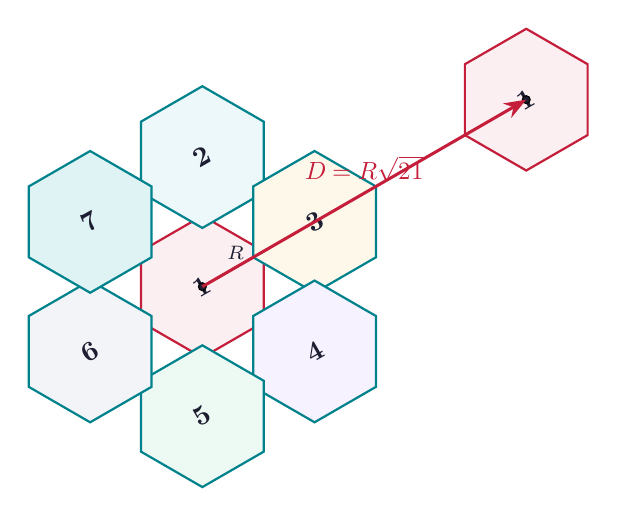
\begin{tikzpicture}[scale=0.95]
  % Define coordinates for 7-cell cluster
  % Centers at distance sqrt(3)*R = 1.732
  \node[hexagon, fill=hdrred!70, draw=myred] (c1) at (0,0) {\textbf{\color{mydark}1}};
  \node[hexagon, fill=hdrteal!50] (c2) at (0, 1.732) {\textbf{\color{mydark}2}};
  \node[hexagon, fill=hdramber!50] (c3) at (1.5, 0.866) {\textbf{\color{mydark}3}};
  \node[hexagon, fill=hdrpurple!50] (c4) at (1.5, -0.866) {\textbf{\color{mydark}4}};
  \node[hexagon, fill=hdrgreen!50] (c5) at (0, -1.732) {\textbf{\color{mydark}5}};
  \node[hexagon, fill=hdrgray!70] (c6) at (-1.5, -0.866) {\textbf{\color{mydark}6}};
  \node[hexagon, fill=hdrteal!90] (c7) at (-1.5, 0.866) {\textbf{\color{mydark}7}};

  % Label showing radius R
  \draw[line, dashed] (0,0) -- (0.9, 0.519) node[midway, above=-1pt, font=\scriptsize] {$R$};
  \draw[fill=mydark] (0,0) circle (1.5pt);

  % Draw a second co-channel cell '1' to show reuse distance D
  % Shift center by i=2, j=1 steps -> distance for N=7 is D = R*sqrt(21) = 4.58R approx 4.0cm
  % Shift: x = R*sqrt(3)*(i + j*cos(60)) = 1.732 * (2 + 0.5) = 4.33, y = R*sqrt(3)*j*sin(60) = 1.732 * 0.866 = 1.5
  \node[hexagon, fill=hdrred!70, draw=myred] (c1_reuse) at (4.33, 2.5) {\textbf{\color{mydark}1}};
  \draw[fill=mydark] (4.33, 2.5) circle (1.5pt);

  % Connect centers with arrow showing D
  \draw[arrow, redarrow, line width=1.1pt] (0,0) -- (4.33, 2.5) node[midway, above, font=\small\bfseries] {$D = R\sqrt{21}$};
\end{tikzpicture}
\end{tcolorbox}

% ===============================================================================
\section{Cell Splitting, Sectoring, and Microcell Zone Concept}
% ===============================================================================

When traffic demand in a cellular network exceeds the capacity of the allocated channels, the network must be densified or modified to support more users. Three primary strategies are used:

\subsection{Cell Splitting}
Cell splitting partitions congested cells into smaller cells (microcells), each with its own base station and a corresponding reduction in transmitter power.
\begin{itemize}[leftmargin=*, itemsep=3pt]
  \item \textbf{Mechanism:} By reducing the cell radius from $R$ to $R/2$, the area of the cell is reduced by a factor of 4. Since each microcell uses the same cluster design, the capacity per unit area increases by a factor of 4.
  \item \textbf{Power Scaling:} To maintain the same co-channel reuse ratio $Q$, the transmit power of the new microcell base stations must be reduced. Power scales as:
    \begin{equation}
      P_{\text{new}} = P_{\text{old}} \cdot \left(\frac{R_{\text{new}}}{R_{\text{old}}}\right)^n = \frac{P_{\text{old}}}{16} \quad (\text{for path loss exponent } n=4)
    \end{equation}
\end{itemize}

\begin{tcolorbox}[tikzbox, title={Cell Splitting Concept (Radius R divided by 2)}]
\centering
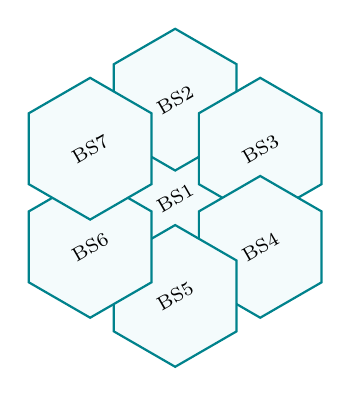
\begin{tikzpicture}[scale=0.8]
  % Original large hexagon
  \node[hexagon, minimum size=3.6cm, fill=none, draw=mydark, dashed, line width=1pt] (h1) at (0,0) {};
  \node at (0, 1.3) {\small Original Cell ($R$)};
  
  % Split hexagons inside
  \node[hexagon, minimum size=1.8cm, fill=hdrteal!30] (s1) at (0,0) {\scriptsize BS1};
  \node[hexagon, minimum size=1.8cm, fill=hdrteal!30] (s2) at (0, 1.558) {\scriptsize BS2};
  \node[hexagon, minimum size=1.8cm, fill=hdrteal!30] (s3) at (1.35, 0.779) {\scriptsize BS3};
  \node[hexagon, minimum size=1.8cm, fill=hdrteal!30] (s4) at (1.35, -0.779) {\scriptsize BS4};
  \node[hexagon, minimum size=1.8cm, fill=hdrteal!30] (s5) at (0, -1.558) {\scriptsize BS5};
  \node[hexagon, minimum size=1.8cm, fill=hdrteal!30] (s6) at (-1.35, -0.779) {\scriptsize BS6};
  \node[hexagon, minimum size=1.8cm, fill=hdrteal!30] (s7) at (-1.35, 0.779) {\scriptsize BS7};
\end{tikzpicture}
\end{tcolorbox}

\subsection{Sectoring}
Instead of omnidirectional antennas, sectoring uses directional antennas at the base station to transmit only in specific directions.
\begin{itemize}[leftmargin=*, itemsep=3.5pt]
  \item \textbf{Principle:} Common configurations are $120^\circ$ sectoring (3 sectors per cell) and $60^\circ$ sectoring (6 sectors per cell).
  \item \textbf{Impact:} By directing transmission, a sector receives interference only from co-channel cells located within its antenna's main beam. This dramatically reduces the number of co-channel interferers, improving the Carrier-to-Interference ratio ($C/I$).
  \item \textbf{Trade-off:} Sectoring divides the channels of a cell into smaller groups, which reduces trunking efficiency and increases handoff frequency.
\end{itemize}

\subsection{Microcell Zone Concept}
To address the trunking efficiency loss and frequent handoffs of sectoring, the microcell zone concept is used.
\begin{itemize}[leftmargin=*, itemsep=3.5pt]
  \item A large cell is divided into three zone transmitters (microcells) located at the periphery, all connected to a single central base station via fiber or microwave link.
  \item As a mobile user moves within the cell, the base station dynamically switches the active zone transmitter. No handoff is triggered at the Mobile Switching Center (MSC) since all zones share the same channels and base station.
\end{itemize}

% ===============================================================================
\section{Channel Assignment and Handoff Strategies}
% ===============================================================================

\subsection{Channel Assignment Strategies}
To optimize spectrum utilization, channels are managed using one of two strategies:
\par\noindent
\begin{tabularx}{\linewidth}{|B{3.2cm}|Y|Y|}
\hline
\rowcolor{hdrgray}
\textbf{Parameter} & \textbf{Fixed Channel Assignment (FCA)} & \textbf{Dynamic Channel Assignment (DCA)} \\
\hline
\textbf{Allocation} & Channels are permanently assigned to each cell according to a reuse plan. & Channels are kept in a central pool and assigned on-demand. \\
\hline
\rowcolor{rowalt}
\textbf{Traffic Adaptability} & Poor. If a cell runs out of channels, calls are blocked, even if adjacent cells are idle. & Excellent. Adapts to real-time spatial traffic variations. \\
\hline
\textbf{Complexity} & Very low. No real-time optimization or coordination required. & High. Requires real-time measurements and central control. \\
\hline
\rowcolor{rowalt}
\textbf{Interference Control} & Hardcoded safety distance protects against co-channel interference. & Requires continuous monitoring of signal levels to avoid collisions. \\
\hline
\end{tabularx}

\subsection{Handoff Strategies}
\begin{tcolorbox}[defbox]
\textbf{Handoff (or Handover):} The process of transferring an active call or data session from one channel or base station to another as the mobile station moves between coverage areas.
\end{tcolorbox}

\begin{enumerate}[label=\textbf{\arabic*.}, leftmargin=*, itemsep=4pt]
  \item \textbf{Hard Handoff ("Break-before-make"):} The mobile station disconnects from the current base station before connecting to the target base station. Used in FDMA and TDMA systems. It is simple but can lead to dropped calls if the connection fails.
  \item \textbf{Soft Handoff ("Make-before-break"):} The mobile station connects to the new base station while maintaining its link with the current base station. Used in CDMA (spread-spectrum) systems. It ensures zero connection gap but consumes double channel resources during the handoff transition.
  \item \textbf{Delayed (or Two-Threshold) Handoff:} Employs a primary signal threshold to initiate handoff, but delays execution until a second, lower threshold is reached. Prevents unnecessary handoffs due to temporary signal fading.
  \item \textbf{Queuing Handoff:} Instead of blocking a handoff request if no channels are available in the target cell, the request is placed in a queue. Since handoff calls have higher priority than new calls, they are served as soon as a channel frees up.
\end{enumerate}

\begin{tcolorbox}[tikzbox, title={Handoff Thresholds and Hysteresis}]
\centering
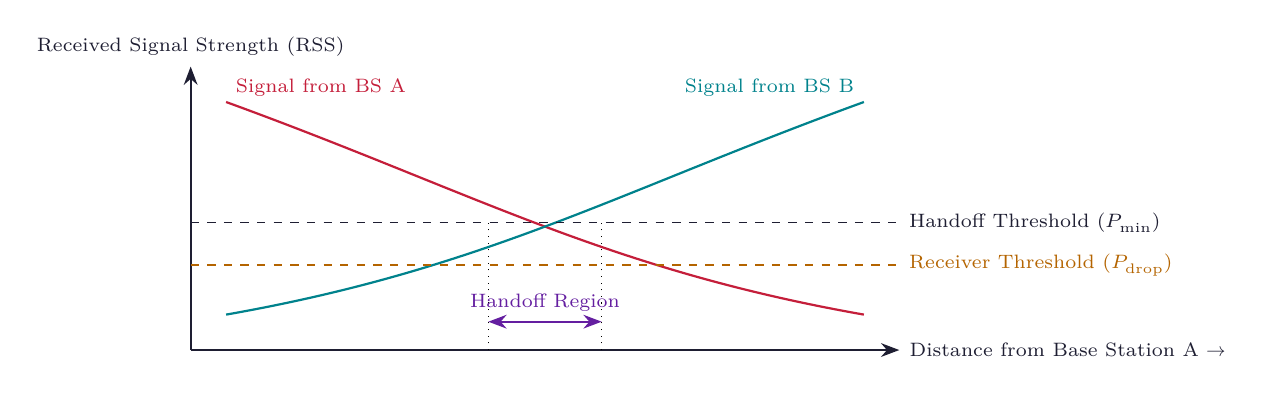
\begin{tikzpicture}[scale=0.9, every node/.style={font=\scriptsize}]
  % Axes
  \draw[arrow] (0,0) -- (10,0) node[right] {Distance from Base Station A $\to$};
  \draw[arrow] (0,0) -- (0,4) node[above] {Received Signal Strength (RSS)};

  % Curves representing signal strength from BS A and BS B
  \draw[thick, color=myred] (0.5, 3.5) to[out=-20, in=170] (9.5, 0.5);
  \node[color=myred, right] at (0.5,3.7) {Signal from BS A};
  
  \draw[thick, color=myteal] (0.5, 0.5) to[out=10, in=-160] (9.5, 3.5);
  \node[color=myteal, left] at (9.5,3.7) {Signal from BS B};

  % Threshold lines
  \draw[dashed, color=mydark] (0, 1.8) -- (10, 1.8) node[right] {Handoff Threshold ($P_{\text{min}}$)};
  \draw[dashed, color=myamber] (0, 1.2) -- (10, 1.2) node[right] {Receiver Threshold ($P_{\text{drop}}$)};

  % Vertical lines for intersections
  \draw[dotted] (4.2, 0) -- (4.2, 1.8);
  \draw[dotted] (5.8, 0) -- (5.8, 1.8);
  
  \draw[thick, Stealth-Stealth, color=mypurple] (4.2, 0.4) -- (5.8, 0.4) node[midway, above] {Handoff Region};
\end{tikzpicture}
\end{tcolorbox}

% ===============================================================================
\section{Interference, Capacity, and Power Control}
% ===============================================================================

\subsection{Co-channel Interference (CCI)}
CCI arises from cells using the same frequency channels. The Carrier-to-Interference ratio ($C/I$) determines signal quality:
\begin{equation}
  \frac{C}{I} = \frac{S}{\sum_{i=1}^{i_0} I_i}
\end{equation}
Where $S$ is the desired signal power and $I_i$ is the interference power from the $i$-th co-channel cell, and $i_0$ is the number of co-channel interferers (first tier).
Assuming propagation path loss follows a power law ($P_r \propto d^{-n}$):
\begin{equation}
  \frac{C}{I} = \frac{R^{-n}}{\sum_{i=1}^{i_0} D_i^{-n}} \approx \frac{(D/R)^n}{i_0} = \frac{(\sqrt{3N})^n}{i_0}
\end{equation}
Where $n$ is the path loss exponent. For a typical first-tier of 6 co-channel interferers ($i_0 = 6$):
\begin{equation}
  \frac{C}{I} \approx \frac{(3N)^{n/2}}{6}
\end{equation}

\subsection{Adjacent Channel Interference (ACI)}
ACI is caused by signals in adjacent frequency bands. It occurs due to imperfect receiver filtering, which allows nearby frequencies to leak into the passband (spectral regrowth).
\begin{itemize}[leftmargin=*, itemsep=2.5pt]
  \item \textbf{Mitigation:} Guard bands are inserted between channel allocations, and adjacent channels are never assigned to the same cell or adjacent cells in the reuse pattern.
\end{itemize}

\subsection{Trunking and Capacity Measures (Erlang)}
Trunking exploits the statistical behavior of users, allowing a small number of channels to serve a much larger user base.
\begin{itemize}[leftmargin=*, itemsep=3pt]
  \item \textbf{Traffic Intensity ($A$):} Measured in \textbf{Erlangs} (dimensionless unit of traffic). For $U$ users, each with call request rate $\lambda$ and average call duration $H$:
    \begin{equation}
      A = U \cdot A_u = U \cdot (\lambda H)
    \end{equation}
  \item \textbf{Erlang B (Blocked Calls Cleared):} Determines the probability of a call being blocked ($P_b$) when no channels are available. Calls are cleared immediately.
    \begin{equation}
      P_b = \frac{\frac{A^C}{C!}}{\sum_{k=0}^{C} \frac{A^k}{k!}} \quad (C = \text{number of channels})
    \end{equation}
  \item \textbf{Erlang C (Blocked Calls Delayed):} Assumes blocked calls enter a queue, calculating the probability of a call experiencing a delay.
\end{itemize}

\subsection{Power Control}
Power control dynamically adjusts the transmitter power of mobile units and base stations.
\begin{itemize}[leftmargin=*, itemsep=3pt]
  \item \textbf{Need:} Solves the \textbf{Near-Far Problem} in CDMA, where a transmitter near the base station overrides weaker signals from distant users.
  \item \textbf{Open-Loop Power Control:} The mobile station estimates path loss based on the received pilot signal and adjusts its transmit power accordingly. It is fast but does not account for independent uplink fading.
  \item \textbf{Closed-Loop Power Control:} The base station measures the received signal SNR from the mobile station and sends power adjustment commands (up/down bits) via the downlink control channel. Highly accurate.
\end{itemize}

\newpage
% ===============================================================================
\section{Wireless Cellular Standards: 2G and 3G}
% ===============================================================================

Cellular networks transitioned from analog voice (1G) to digital systems (2G) and high-speed data networks (3G):

\par\noindent
\begin{tabularx}{\linewidth}{|B{3.2cm}|Y|Y|}
\hline
\rowcolor{hdrteal}
\textbf{Feature} & \textbf{2G Cellular Standards} & \textbf{3G Cellular Standards} \\
\hline
\textbf{Primary Standards} & \textbf{GSM} (Global System for Mobile) and \textbf{IS-95} (cdmaOne). & \textbf{WCDMA} (UMTS) and \textbf{CDMA2000}. \\
\hline
\rowcolor{rowalt}
\textbf{Access Scheme} & TDMA/FDMA (GSM), CDMA (IS-95). & WCDMA (DS-CDMA), CDMA2000. \\
\hline
\textbf{Channel Bandwidth} & 200 kHz (GSM), 1.25 MHz (IS-95). & 5 MHz (WCDMA), 1.25 MHz (CDMA2000). \\
\hline
\rowcolor{rowalt}
\textbf{Data Rate} & 9.6 kbps (GSM), up to 144 kbps (IS-95B). & 384 kbps (UMTS) up to 2 Mbps (HSPA). \\
\hline
\textbf{Voice/Data Type} & Digital voice, SMS, basic packet data (GPRS). & High-speed packet data, video calling, mobile internet. \\
\hline
\rowcolor{rowalt}
\textbf{Modulation} & GMSK (GSM), BPSK/QPSK (IS-95). & QPSK/16-QAM. \\
\hline
\end{tabularx}

\subsection{Evolutionary Paths}
\begin{itemize}[leftmargin=*, itemsep=3pt]
  \item \textbf{GSM to 3G:} GSM (9.6 kbps) $\to$ GPRS (General Packet Radio Service, 115 kbps) $\to$ EDGE (Enhanced Data Rates for GSM Evolution, 384 kbps, uses 8-PSK) $\to$ WCDMA/UMTS (2 Mbps).
  \item \textbf{IS-95 to 3G:} IS-95A $\to$ IS-95B $\to$ CDMA2000 1xRTT $\to$ CDMA2000 1xEV-DO (Evolution-Data Optimized).
\end{itemize}

% ===============================================================================
% MANDATORY QUICK REVISION PAGE
% ===============================================================================
\newpage
\begin{center}
  {\large\bfseries\color{myred} Quick Revision --- Module I}\\[3pt]
  {\small\color{mydark} Cellular Concepts and Wireless Standards $|$ PE-EC701C}
\end{center}
\noindent{\color{myred}\rule{\linewidth}{1.2pt}}
\vspace{4pt}

\begin{tcolorbox}[formulabox, title={\textbf{Key Formulas at a Glance}}]
\renewcommand{\arraystretch}{1.3}
\begin{tabularx}{\linewidth}{B{5.5cm} X}
System Capacity & $C = M \cdot S = M \cdot k \cdot N$ \\
Cluster Size Relation & $N = i^2 + ij + j^2$ \\
Co-channel Reuse Distance & $D = R \sqrt{3N}$ \\
Co-channel Reuse Ratio & $Q = \frac{D}{R} = \sqrt{3N}$ \\
Carrier-to-Interference Ratio ($C/I$) & $\frac{C}{I} \approx \frac{(\sqrt{3N})^n}{i_0} = \frac{(3N)^{n/2}}{6}$ \quad (assuming $i_0 = 6$ interferers) \\
Microcell Power Scaling & $P_{\text{new}} = P_{\text{old}} \cdot \left(\frac{R_{\text{new}}}{R_{\text{old}}}\right)^n$ \\
Traffic Intensity (Erlangs) & $A = U \cdot \lambda \cdot H$ \\
Erlang B Equation & $P_b = \frac{A^C/C!}{\sum_{k=0}^{C} A^k/k!}$
\end{tabularx}
\end{tcolorbox}

\begin{tcolorbox}[defbox, title={\textbf{One-Line Definitions}}]
\begin{itemize}[leftmargin=*, itemsep=2.5pt, topsep=0pt]
  \item \textbf{Frequency Reuse:} Reassigning the same channel group to cells separated by a safe distance $D$.
  \item \textbf{Cell Splitting:} Subdividing congested cells into smaller microcells to increase capacity.
  \item \textbf{Sectoring:} Replacing omnidirectional antennas with directional ones to focus energy and reduce interference.
  \item \textbf{Near-Far Problem:} Interference caused when a mobile user near the BS drowns out weaker signals from distant users.
  \item \textbf{Trunking:} Concentrating a large user base onto a smaller pool of shared channels using statistical demand.
  \item \textbf{Hard Handoff:} Break-before-make switch where connection to the current cell is severed before joining the next.
  \item \textbf{Soft Handoff:} Make-before-break switch maintaining links to both old and new BSs simultaneously during transition.
  \item \textbf{Erlang B:} A formula representing traffic blockage probability under a blocked-calls-cleared assumption.
\end{itemize}
\end{tcolorbox}

\begin{tcolorbox}[exambox, title={\textbf{Frequently Asked / Viva Questions}}]
\begin{enumerate}[topsep=0pt, label=\textbf{Q\arabic*.}, itemsep=5pt]
  \item \Q{Why is a hexagonal cell shape preferred over a square or triangle?}
    It provides the closest approximation to a circular radiation pattern, tiles the plane without gaps or overlaps, and maximizes cell area for a given radius, minimizing base station count.
  \item \Q{Derive the relation between cluster size $N$ and reuse distance $D$.}
    In a hexagonal grid, the distance between adjacent cells is $R\sqrt{3}$. Stepping $i$ times along one axis and $j$ times along another rotated by $60^\circ$ gives $D = R\sqrt{3(i^2 + ij + j^2)} = R\sqrt{3N}$.
  \item \Q{Explain the Near-Far problem and how it is resolved.}
    A mobile station close to the base station transmits signals that arrive with much higher power than a distant station, drowning it out. It is resolved by closed-loop power control.
  \item \Q{How does cell splitting increase system capacity?}
    By reducing the cell radius by half, the area of each cell decreases to one-fourth. Replicating the channel groups across these smaller cells increases the channel density per unit area fourfold.
  \item \Q{What are the typical values of cluster size $N$? Why can $N$ not be any arbitrary integer?}
    $N = i^2 + ij + j^2$. For integers $i$ and $j$, $N$ can only be 1, 3, 4, 7, 9, 12, 19, 21, etc. Other values cannot tile a hexagonal grid without leaving gaps.
  \item \Q{State the main difference between Erlang B and Erlang C.}
    Erlang B assumes blocked calls are cleared immediately (no queue). Erlang C assumes blocked calls enter a queue and wait until a channel is freed.
  \item \Q{Contrast hard handoff and soft handoff.}
    Hard handoff is "break-before-make" (link broken first; used in TDMA/FDMA). Soft handoff is "make-before-break" (simultaneous links; used in CDMA).
  \item \Q{Explain how sectoring improves the $C/I$ ratio.}
    Directional antennas limit transmission/reception angles. A $120^\circ$ sector receives interference from only 2 of the 6 co-channel interferers in the first tier, boosting $C/I$ without changing $N$.
  \item \Q{What is the microcell zone concept?}
    A design where a cell's channels are shared across three peripheral zones connected to a single BS. Handoffs between zones are handled locally, avoiding MSC loading.
  \item \Q{Identify the key parameters of the GSM standard.}
    It is a 2G standard using TDMA/FDMA, with 200 kHz channels, GMSK modulation, and a maximum user data rate of 9.6 kbps.
  \item \Q{What is GPRS and how does it relate to GSM?}
    General Packet Radio Service (GPRS) is a 2.5G packet-switched extension to the circuit-switched GSM network, allowing data rates up to 115 kbps.
  \item \Q{Define Grade of Service (GoS).}
    A metric representing the probability of a call being blocked (Erlang B) or delayed beyond a threshold (Erlang C) during the busy hour.
\end{enumerate}
\tcbset{colbacktitle=myteal, coltitle=white}
\end{tcolorbox}

\begin{tcolorbox}[tikzbox, title={Comparison of 2G and 3G Cellular Technologies}]
\renewcommand{\arraystretch}{1.4}
\par\noindent
\begin{tabularx}{\linewidth}{|B{3.0cm}|Y|Y|}
\hline
\rowcolor{hdrgray}
\textbf{Parameter} & \textbf{\color{myteal}2G (GSM / IS-95)} & \textbf{\color{myred}3G (WCDMA / CDMA2000)} \\
\hline
\textbf{Primary Service} & Digital voice transmission and SMS. & High-speed packet data, mobile internet. \\
\hline
\textbf{Channel Width} & 200 kHz (GSM), 1.25 MHz (IS-95). & 5.0 MHz (WCDMA), 1.25 MHz (CDMA2000). \\
\hline
\rowcolor{rowalt}
\textbf{Modulation} & GMSK, BPSK. & QPSK, 16-QAM (in HSPA). \\
\hline
\textbf{Key Limit} & Strict capacity limits, low data rates. & High hardware cost, complex power control. \\
\hline
\end{tabularx}
\end{tcolorbox}

\end{document}
